\documentclass[11pt]{article}

%Both greek and english language support
\usepackage[greek,english]{babel}
\usepackage{alphabeta}
\usepackage[utf8]{inputenc}

% For \includegraphics
\usepackage{graphicx}   
\usepackage[space]{grffile}

% Maths extra
\usepackage{amsmath}

%Todo notes
% \usepackage[colorinlistoftodos]{todonotes}

% Page margins 
\usepackage{geometry}
 \geometry{
 a4paper,
 total={170mm,257mm},
 left=20mm,
 top=20mm,
 }

%Negative exponential
\DeclareUnicodeCharacter{2212}{-}   

\begin{document}
%--------------------------------------------------------------------------------------------
% Title Page
\begin{titlepage}
    \center
    %----------------------------------------------------------------------------------------
    %	HEADING SECTIONS
    \textsc{\LARGE Technical University of Crete}\\[2cm] 
    \Large Ψηφιακή Επεξεργασία Σήματος\\
    \emph{ΤΗΛ302}\\[1cm] 
    
    \rule{\linewidth}{0.5mm} \\[0.5cm]
        { \huge \bfseries Εργαστήριο 2}\\[0.5cm]
    \rule{\linewidth}{0.5mm} \\[2.5cm]
    
    \begin{minipage}{0.4\textwidth}
        \begin{flushleft} \large
            \emph{Authors:}\\
                Ισίδωρος Πατεράκης AM: 2017030091
                Μαρίνου Ιωάννα AM: 2016030143
                Σπυριδάκης Χρήστος AM: 2014030022
        \end{flushleft}
    \end{minipage}
    ~
    \begin{minipage}{0.4\textwidth}
        \begin{flushright} \large
            LAB30242846 \\
        \end{flushright}
    \end{minipage}\\[2cm]
    
    {\large November 12, 2019}\\[2cm] 
    %----------------------------------------------------------------------------------------
    %	LOGO
    
\includegraphics[scale=0.5]{TUC.png} 
    \vfill
\end{titlepage}

%---------------------------------------------------------------------------------------------
%   Exercise 1
\section*{Άσκηση 1}
Αρχικά το σύστημα το οποίο μας δίνεται απεικονίζεται παρακάτω, ενώ ξέρουμε ότι είναι ένα αιτιατό, γραμμικό και αμετάβλητο κατά τη μετατόπιση. Επίσης γνωρίζουμε ότι για τη συχνότητα δειγματοληψίας ισχύει ότι $f_s=1Hz$. Τέλος, γνωρίζουμε ότι το $G_1(z)$ περιγράφεται από την εξίσωση διαφορών $k(n) = 0.9k(n-1)+0.2x(n)$ και το $G_2(z)=\frac{1}{z+0.2}$.

\begin{center}{}
    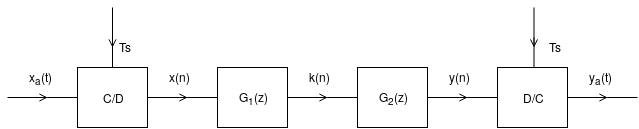
\includegraphics[scale=0.6]{photos/system-diagram.png} \\
    \textbf{Image 1.1:} Given system
\end{center}

%------------------------------------------------------------
%   a
\subsection*{a)}
Για το πρώτο μέρος σχετικά με εύρεση της συνάρτησης μεταφοράς γνωρίζουμε ότι ισχύει:

% Συνάρτηση μεταφοράς
\begin{align}
    \boxed{H(z)=\frac{Y(z)}{X(z)}} \label{tranf_func}
\end{align}

\par \noindent
Μη γνωρίζοντας άμεσα ούτε το $Y(z)$ ούτε το $X(z)$ πρέπει να βρούμε μέσα από τα δεδομένα ένα τρόπο να τα υπολογίσουμε. Ξέρουμε όμως ότι συνελίξεις στο πεδίο του χρόνου είναι πολλαπλασιασμοί στο πεδίο Ζ οπότε βλέπουμε ότι ισχύει:

% Συνελίξεις στο χρόνο -> πολλαπλασιασμοί στο Z
\begin{align}
    X(z)*G_1(z)=K(z) \Rightarrow \boxed{X(z) = \frac{K(z)}{G_1(z)}} \label{first_conv} \\
    K(z)*G_2(z)=Y(z) \Rightarrow \boxed{Y(z) = K(z)G_2(z)} \label{second_conv}
\end{align}

\par \noindent
Από τις εξισώσεις (\ref{tranf_func}) , (\ref{first_conv}) και (\ref{second_conv}) βλέπουμε ότι για την συνάρτηση μεταφοράς ισχύει:

% Από τις παραπάνω που καταλήγουμε για τη συνάρτηση μεταφοράς
\begin{align}
    H(z)&=\frac{K(z)G_2(z)}{\frac{K(z)}{G_1(z)}} \nonumber \\ 
        &=\boxed{G_1(z)G_2(z)} \label{tranf_func_final}
\end{align}

\par \noindent
Το $G_2(z)$ μας δίνεται, οπότε πρέπει να υπολογίσουμε και το $G_1(z)$. Πρώτο βήμα είναι να δημιουργούμε τον Z-Transform του k(n).
\[ K(z)=0.9z^{-1}K(Z)+0.2X(z) \Rightarrow \]

\begin{align}
    \boxed{K(z)=\frac{0.2X(z)}{1-0.9z^{-1}}} \label{k_z_transf}
\end{align}

\par \noindent
Αυτό που παρατηρούμε είναι ότι στην (\ref{k_z_transf}) εμφανίζεται το $X(z)$ συνεπώς από την (\ref{k_z_transf}) και (\ref{first_conv}) καταλήγουμε ότι:

\begin{align}
    \boxed{G_1(z)=\frac{0.2}{1-0.9z^{-1}}} \label{g_1}
\end{align}

\par \noindent
Πλέον έχουμε ότι χρειαζόμαστε για τον υπολογισμό της συνάρτησης μεταφοράς, δηλαδή το $G_1(z)$ και το $G_2(z)$ άρα:

\begin{align}
    H(z)&=G_1(z)G_2(z) \nonumber \\
    &=\frac{0.2}{1-0.9z^{-1}}*\frac{1}{z+0.2} \nonumber \\
    &=\frac{0.2}{(1-0.9z^{-1})(z+0.2)} \nonumber \\
    &=\frac{0.2}{z-0.9+0.2-0.18z^{-1}} \nonumber \\
    &=\frac{0.2}{z-0.7-0.18z^{-1}} \nonumber \\
    &=\boxed{\frac{0.2z^{-1}}{1-0.7z^{-1}-0.18z^{-2}}}
\end{align}

\par \noindent
Όσον αφορά την εξίσωση διαφορών προκύπτει ότι:
\[ H(z)=\frac{Y(z)}{X(z)}=\frac{0.2z^{-1}}{1-0.7z^{-1}-0.18z^{-2}} \Leftrightarrow \]
\[ Y(z) - 0.7z^{-1}Y(z) -0.18z^{-2}Y(z) = 0.2z^{-1}X(z) \]

\par \noindent
Άρα από τον αντίθετο μετασχηματισμό Z καταλήγουμε ότι:
\[ y(n) - 0.7y(n-1) -0.18y(n-2) = 0.2x(n-1) \Leftrightarrow \]
\begin{align}
    \boxed{y(n) = 0.7y(n-1) + 0.18y(n-2) + 0.2x(n-1)}
\end{align}

%------------------------------------------------------------
%   b
\subsection*{b)}
Αφού είχαμε βρει την συνάρτηση μεταφοράς, μπορούσαμε να σχεδιάσουμε το διάγραμμα πόλων - μηδενικών με την χρήση του MATLAB.

\begin{center}{}
    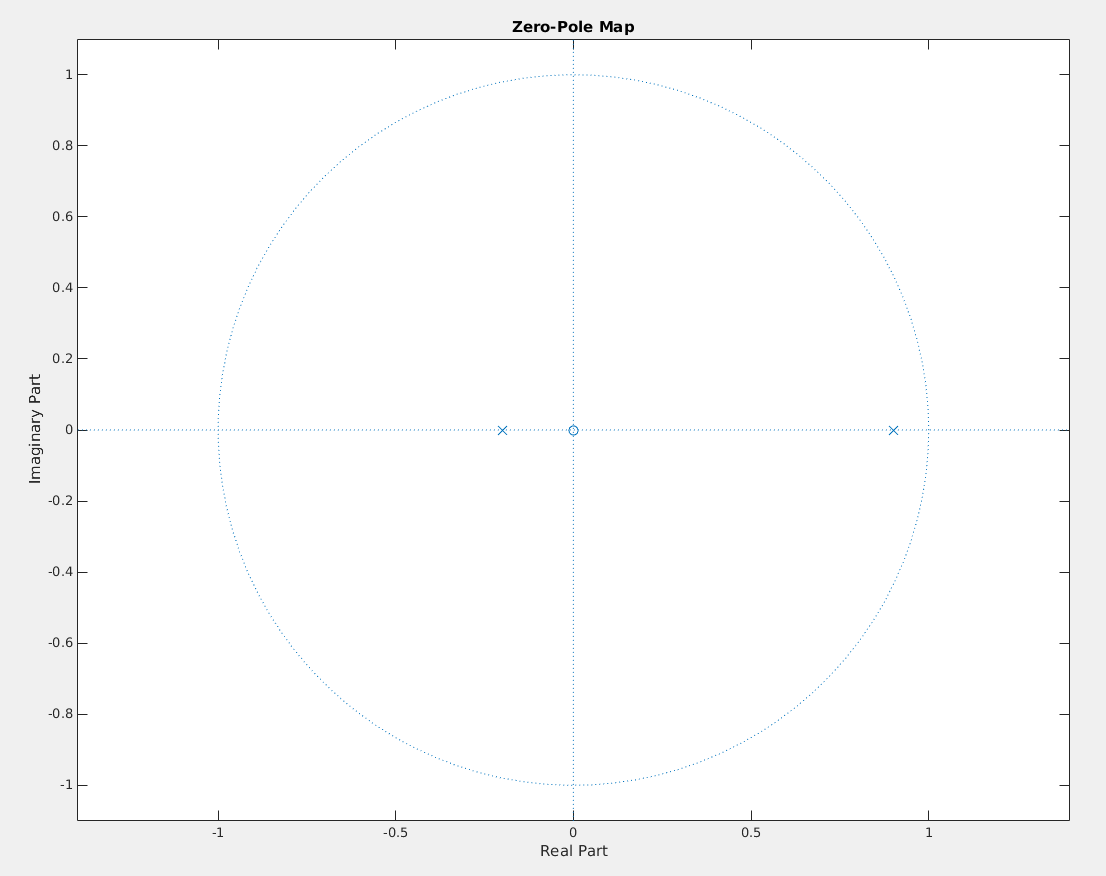
\includegraphics[scale=0.35]{photos/Zero_Pole_Map.png}\\
    \textbf{Image 1.2:} Pole-Zero map on Matlab
\end{center}

%------------------------------------------------------------
%   c
\subsection*{c)} 
Για να είναι BIBO ευσταθές το σύστημα, όπως έχουμε δει και από την θεωρία πρέπει να ισχύει ότι ο ROC (Region of convergence) περιλαμβάνει το μοναδιαίο κύκλο $(|z|=1)$. Επίσης ξέρουμε ότι το σύστημα είναι αιτιατό πράγμα που σημαίνει ότι είναι σίγουρα δεξιόπλευρο. Άρα η περιοχή σύγκλισης του ξεκινάει από ένα κύκλο και εκτείνεται προς το $\pm \infty$. 
\par \noindent
Συνεπώς $|z|>|r_1|$, με την χρήση του σχεδιάγραμμα μηδενικών - πόλων του παραπάνω ερωτήματος βλέπουμε ότι η τιμή του $r_1=0.9$ πράγμα που σημαίνει ότι περιλαμβάνεται ο μοναδιαίος κύκλος άρα το σύστημα είναι BIBO ευσταθές.

%------------------------------------------------------------
%   d
\subsection*{d)}

%------------------------------------------------------------
%   f
\subsection*{f)}


%---------------------------------------------------------------------------------------------
%   Exercise 2
\section*{Άσκηση 2}
Δίνεται η συνάρτηση μεταφοράς:

$$H(z) = \frac{ 4 - 3.5z^{-1}}{1 - 2.5z^{-1} + z^{-2} } , |z| > 2$$

%------------------------------------------------------------
%   a
\subsection*{a)}
Η θεωρητική ανάλυση της συνάρτησης μεταφοράς είναι η εξής:
\par \noindent
Βρίσκονται οι πόλοι λύνοντας την δευτεροβάθμια εξίσωση.
Σπάει ο αριθμητής και βρίσκονται οι συντελεστές του μέσω της μεθόδου χρήσης των Α-Β.

\[ 1 - 2.5z^{-1} + z^{-2} = 0 \]
\[ Δ = β^2-4αγ = (-2.5)^2-4*1*1 = 6.25 - 4 = 2.25 \]
\[ \sqrt{Δ} = \sqrt{2.25} = 1.5 \]
\[ p_{1,2} = \frac{2.5 \pm \sqrt{Δ}}{2} = \frac{2.5\pm1.5}{2} \Rightarrow p_1=2 \quad \textrm{and} \quad p_2=0.5 \]


\begin{align*}
    \frac{4-3.5z^{-1}}{1-2.5z^{-1}+z^{-2}} &= \frac{A}{1-p_{1}z^{-1}} + \frac{B}{1-p_{2}z^{-1}} \\
    &=\frac{A}{1-2z^{-1}} + \frac{B}{1-0.5z^{-1}} \\
    &=\frac{A(1-0.5z^{-1}) + B(1-2z^{-1})}{(1-2z^{-1})(1-0.5z^{-1})} \Leftrightarrow \\
    & A(1-0.5z^{-1}) + B(1-2z^{-1})=4-3.5z^{-1} \Leftrightarrow \\
    & A - 0.5Az^{-1} + B -2Bz^{-1} = 4 -3.5z^{-1} \Leftrightarrow \\
    & A + B - (0.5A + 2B) = 4 -3.5z^{-1}
\end{align*}

\par \noindent
Συνεπώς:
\[ A+B=4 \Leftrightarrow A=4-B \]
\[ 0.5A+2B=3.5 \Leftrightarrow  A+4B=7 \Leftrightarrow  4-B+4B=7 \Leftrightarrow  3B=3 \Rightarrow  B=1 \quad \textrm{and} \quad  A=3 \]

\par \noindent
Άρα:
$$H(z) =\frac{3}{1-2z^{-1}} + \frac{1}{1-0.5z^{-1}} $$ 

\par \noindent
Το αποτέλεσμα επαληθεύεται μέσω MATLAB:
\begin{center}{}
    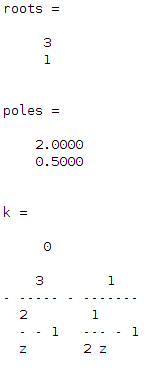
\includegraphics[scale=0.6]{photos/roots_poles_k.png} \\
    \textbf{Image 2.1:} Matlab result 
\end{center}

%------------------------------------------------------------
%   b
\subsection*{b)}
Το σύστημα είναι αιτιατό για $|z| > 2$.
Για δεξιόπλευρο όρο ισχύει η ιδιότητα:

\[
       \frac{K_i*Z}{Z-A_i} \Longleftrightarrow K_i*(A_i^n)*u(n)
\] 

\par \noindent
Οπότε προκύπτει το αποτέλεσμα:

\[
    3*(2^n)*u(n) + (0.5^n)u(n)
\] 

\par \noindent
Το αποτέλεσμα επαληθεύεται μέσω MATLAB:

\begin{center}{}
    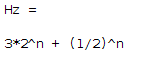
\includegraphics[scale=0.7]{photos/H_z.png} \\
    \textbf{Image 2.2:} Matlab result 
\end{center}

\end{document}